\documentclass{BeamerTemplate}
\title{Module 7 - Estimation ponctuelle et lois échantillonnales}
\subtitle{STT-1000 Probabilités et statistique}

\usepackage{adjustbox}


\begin{document}
\AtBeginSection{\frame{\sectionpage}}

\begin{frame}

\titlepage

\end{frame}

\section{Concepts d'inférence statistique}


\begin{frame}[t]{L'inférence statistique}

Tirer des conclusions au sujet d'une population à l'aide d'un échantillon.\\

\begin{itemize}\itemsep 5mm
\item<2-> Faire rouler sur un circuit 20 voitures neuves prises au hasard
%parmi celles qui sortent d'une usine
afin d'étudier la fiabilité de la suspension.
\item<2-> Sonder une population d'acheteurs potentiels d'un
nouveau produit sur l'attrait d'une option.

\centerline{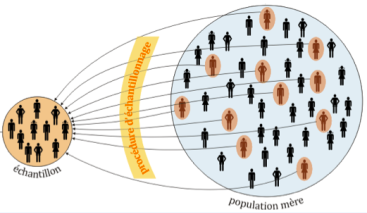
\includegraphics[width=5cm]{pop.png}}
\tiny
\href{http://www.educatim.fr/tq/co/Module_TQ_web/co/population.html}{www.educatim.fr/tq/co/Module\_TQ\_web}

\end{itemize}
\end{frame}

\begin{frame}[t]{Deux types d'inférence}

\begin{tabular}{p{5cm}|p{5cm}}
{\bf Estimation de paramètres}&{\bf Vérification d'hypothèses}\\\hline

\uncover<2->{\alerter{Estimation ponctuelle:} }& \uncover<4->{\alerter{Tests d'hypothèses:} }\\[3mm]
\uncover<2->{$\bullet\;\mu$ estimé par...}&\uncover<4->{$\bullet\;$ A-t-on $\;\mu\leq60$?} \\[3mm]
\uncover<2->{$\bullet\;\sigma^2$ estimé par...}&\uncover<4->{$\bullet\;$ A-t-on $\;\sigma^2<10$?}\\[3mm]\cline{1-1}
\uncover<3->{\alerter{Intervalles de confiance: }}&\uncover<4->{$\bullet\;$ A-t-on $\;\mu_1=\mu_2=\mu_3 $?}\\[3mm]
\uncover<3->{associer une marge d'erreur}&\\[-1mm]
\uncover<3->{aux estimations ponctuelles}
\end{tabular}

\end{frame}

\begin{frame}[t]{Modèle, loi, paramètres}
\centerline{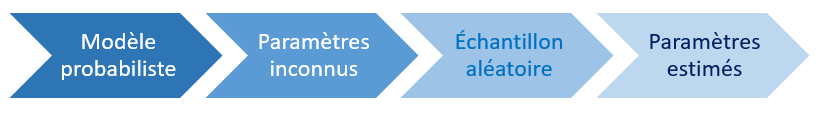
\includegraphics[width=11cm]{estimation.png}}

\end{frame}

\begin{frame}[t]{Exemple 1: masse des camions}

{\small
\begin{tabular}{l p{5cm}}
 {\bf Population :}& l'ensemble des camions qui passent sur un viaduc\\[3mm]
{\bf Caractéristique d'intérêt:}   &  $X$: masse d'un camion\\[3mm]
{\bf Modèle probabiliste :}& $X\sim \mathcal{N}(\mu,\sigma^2)$\\[3mm]
{\bf Paramètre d'intérêt :}&  $\mu$: masse
moyenne des camions  sur ce viaduc\\[3mm]
{\bf Taille d'échantillon: }&  $n=25$\\[3mm]
{\bf Échantillon aléatoire:}&  $X_1,\,X_2,...,\,X_{25}$\\[3mm]
{\bf Échantillon observé:}&  $x_1,\,x_2,...,\,x_{25}$\\[3mm]
{\bf Estimation ponctuelle :} &$\overline x = 16,5$ tonnes
\end{tabular}
}
\end{frame}


\section{Estimation ponctuelle}



\begin{frame}[t]{Paramètres classiques: $\mu$ et $\sigma^2$}

\begin{itemize}\itemsep4mm
\item<1-> Par quelles quantités pourrait-on estimer la moyenne et la variance de la population?\\


\uncover<2->{\it Par \alerter{$\overline X$} et \alerter{$S^2$}\hfill }
\item<3-> Ces mesures échantillonnales sont-elles des variables aléatoires?\\

\item<4-> Elles ont donc une loi de probabilité...
\end{itemize}
\end{frame}

\begin{frame}[t]{Exemple 2: simulation de données}

Prenons un échantillon de 25 camions et mesurons leur masse (distribuée selon le modèle normal). On s'attend à ce que $\overline x$ diffère un peu de $\mu$.

\begin{center}
    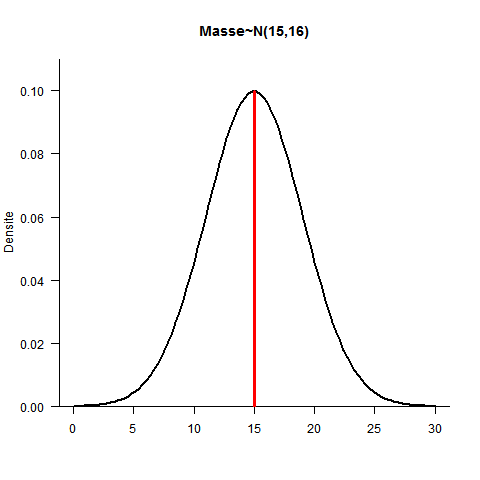
\includegraphics[width=5cm]{modele.png}

\end{center}

\end{frame}

\begin{frame}[t]{Exemple 2: Et si on recommençait 1000 fois?}

{\small  Comment seraient distribuées nos 1000 moyennes(chaque fois avec $n=25$)? }

\begin{center}
    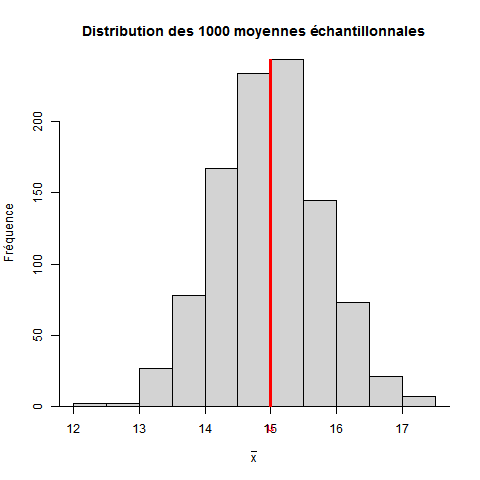
\includegraphics[width=5cm]{moy1000.png}

\end{center}

\end{frame}

\begin{frame}[t]{Exemple 2: Si on changeait la taille d'échantillon?}

{\small Qu'adviendrait-il de la distribution des $\overline x$ avec un $n$ différent?}\\

\begin{center}
    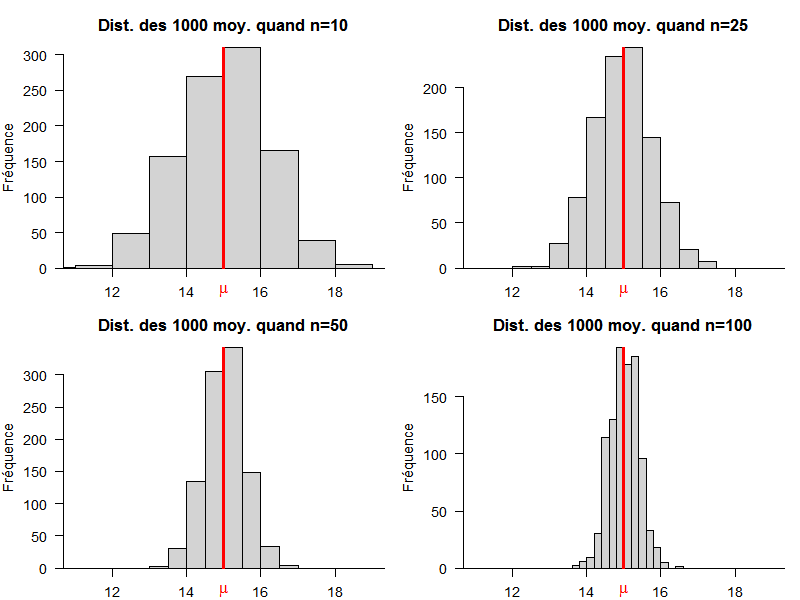
\includegraphics[width=8cm]{moyennes.png}

\end{center}
\end{frame}




\begin{frame}[t]{Qualités d'un estimateur}

 Le choix de \alerter{$\overline X$} et \alerter{$S^2$} est-il le meilleur pour estimer $\mu$ et $\sigma^2$? \\
 Quelles qualités devrait avoir un bon estimateur?\\

\begin{enumerate}\itemsep1cm
\item<1-> Être \alerter{sans biais}, i.e. avoir une valeur espérée égale au paramètre estimé.
\item<2-> Avoir une \alerter{variance faible}, idéalement qui diminue lorsque $n$ grandit.
\end{enumerate}
\end{frame}

\begin{frame}[t]{Estimation de l'espérance $\mu$ par $\overline{X}$}
Soit $X_1,\ldots,X_n$ des variables aléatoires indépendantes d'espérance $\mu$ et de
variance $\sigma^2$. \\
Alors $ \overline{X} = \dfrac1n \sum\limits_{i=1}^{n}X_i$ est-il un bon estimateur de $\mu$?

\begin{itemize}
\item<1-> \alerter{$\overline{X}$ est-il sans biais?} 
\vfill

\item<2-> \alerter{$V(\overline{X})$ diminue-t-elle quand $n$ augmente?} 

\vfill
%\item<3-> $EQM(\hat{M} ) = \sigma^2/n$
\end{itemize}
\end{frame}


\begin{frame}[t]{Estimation d'une variance $\sigma^2$ par $S^2$}

Soit $X_1,\ldots,X_n$ des variables aléatoires indépendantes d'espérance $\mu$ et de
variance $\sigma^2$. \\
${S}^2 = \dfrac{1}{n-1}\sum\limits_{i=1}^{n}(X_i-\overline{X})^2$ est-il bon un estimateur de $\sigma^2$?

\begin{itemize}
\item<1-> \alerter{${S}^2$ est-il sans biais?}
\vfill

\item<2-> \alerter{$V({S}^2)$ diminue-t-elle quand $n$ augmente?} 

\uncover<2->{On montrera plus tard que si les $X_i$ proviennent d'une loi normale, la variance de ${S}^2$ est $$V(S^2)=\dfrac{2\sigma^4}{n-1}.$$}
\end{itemize}

\end{frame}


\begin{frame}[t]
\begin{itemize}
\item Les hommes canadiens mesurent en moyenne 1,78 m. Supposons $X\sim\mathcal{N}(1,78; \sigma^2)$.
\item Jacques mesure 250 Canadiens choisis au hasard.
\item Marie mesure 1000 Canadiens choisis au hasard.
\end{itemize}
\bigskip

{\bf Vrai ou Faux?}
\medskip

Jacques a plus de chances que Marie d'obtenir...
\begin{itemize}
\item  une taille moyenne supérieure à 1,78 m.
\item  une taille moyenne supérieure à 1,82 m.
\end{itemize}


\vspace{1cm}

\end{frame}
%%%%%%%%%%%%%%%%%%%%%%%%%%%%%%%%%%%%%%%%%%%%%%%%%%%%%%%%%%%%%%%%%%%%%%%%%%

\section{Lois échantillonnales}

\begin{frame}[t]{Distribution de certaines statistiques}
\begin{enumerate}[$\bullet$]
\item Les estimateurs sont des variables aléatoires.
\item Leur distribution dépend souvent de la loi de $X$ dans la population.
\item Pour associer une marge d'erreur à un estimateur, on doit trouver sa loi.
\item Les lois qui impliquent des estimateurs sont appelées des {\it distributions échantillonnales}. Nous en verrons trois:

    \begin{itemize}\itemsep1mm
\item Normale $\mathcal{N}(\mu, \sigma^2/n)$
\item Student $\;\;t_v$
\item Khi-carré $\chi^2_v$
\end{itemize}
\end{enumerate}

\end{frame}

\begin{frame}[t]{Distribution de certaines statistiques}
Dans le cas o\`u $X_1,\ldots,X_n\sim \mathcal{N}(\mu,\sigma^2)$ indépendantes (i.i.d.), \\
on connaît la loi de plusieurs statistiques.

\medskip

\begin{itemize}\itemsep3mm
\item {$\overline{X}\sim \mathcal{N}\left(\mu,\frac{\sigma^2}{n}\right)$}

\item {$\dfrac{\overline{X}-\mu}{\sigma/\sqrt{n}}\sim \mathcal{N}(0,1)$}

\item {$\dfrac{\overline{X}-\mu}{S/\sqrt{n}}\sim t_{n-1}$}

\item {$\dfrac{(n-1)S^2}{\sigma^2}\sim \chi^2_{n-1}$}

\end{itemize}


\end{frame}

\section{Loi du khi-carré}

\begin{frame}[t]{Loi du khi-deux (ou loi du khi-carré)}
\begin{itemize}
\item valeurs possibles d'une variable suivant une $\chi^2_v$ : $[0,\infty)$ 
\item un seul paramètre qu'on appelle "degrés de liberté".
\end{itemize}

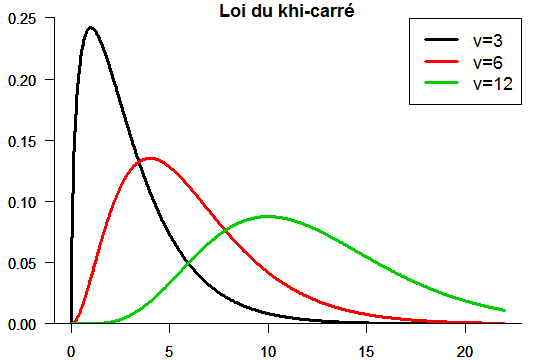
\includegraphics[width=7.5cm]{khi.png}
\end{frame}

\begin{frame}[t]{Propriétés de la loi du khi-carré}

{\small
\begin{itemize}\itemsep2mm
\item<1-> Si $K\sim\chi^2_v$, alors $\left\{\begin{array}{ll}E(K)& = v\\V(K) &= 2v
    \end{array}\right.$
\item<2-> Si $Z\sim \mathcal{N}(0,1)$, alors $Z^2\sim\chi^2_1$ %[et donc si $Z\sim \mathcal{N}(\mu,\sigma^2)$ et $X = \{(Z-\mu)/\sigma\}^2$, alors $X\sim\chi^2_1$].
\item<2-> Si $K_1,\ldots,K_n$ sont des v.a. indépendantes et que $K_i\sim\chi^2_{v_i}$, alors $$K_1+\cdots+K_n\sim\chi^2_{v_1+\cdots+v_n}$$
\item<3-> Si $X_1,\ldots,X_n$ sont i.i.d. $\mathcal{N}(\mu,\sigma^2)$, alors $$\dfrac{\sum_{i=1}^n(X_i-\mu)^2}{\sigma^2}\sim\chi^2_n\qquad \text{et}\qquad\frac{(n-1)S^2}{\sigma^2}\sim\chi^2_{n-1}$$
\end{itemize}
}
\end{frame}
\begin{frame}[t]{Table de la loi du khi-deux}


\begin{minipage}[b]{2.5cm}{
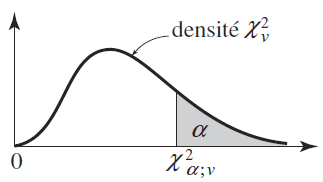
\includegraphics[width=2.5cm]{khi-fig.png}

\vspace{9cm}}
\end{minipage}
\begin{minipage}[b]{7.6cm}{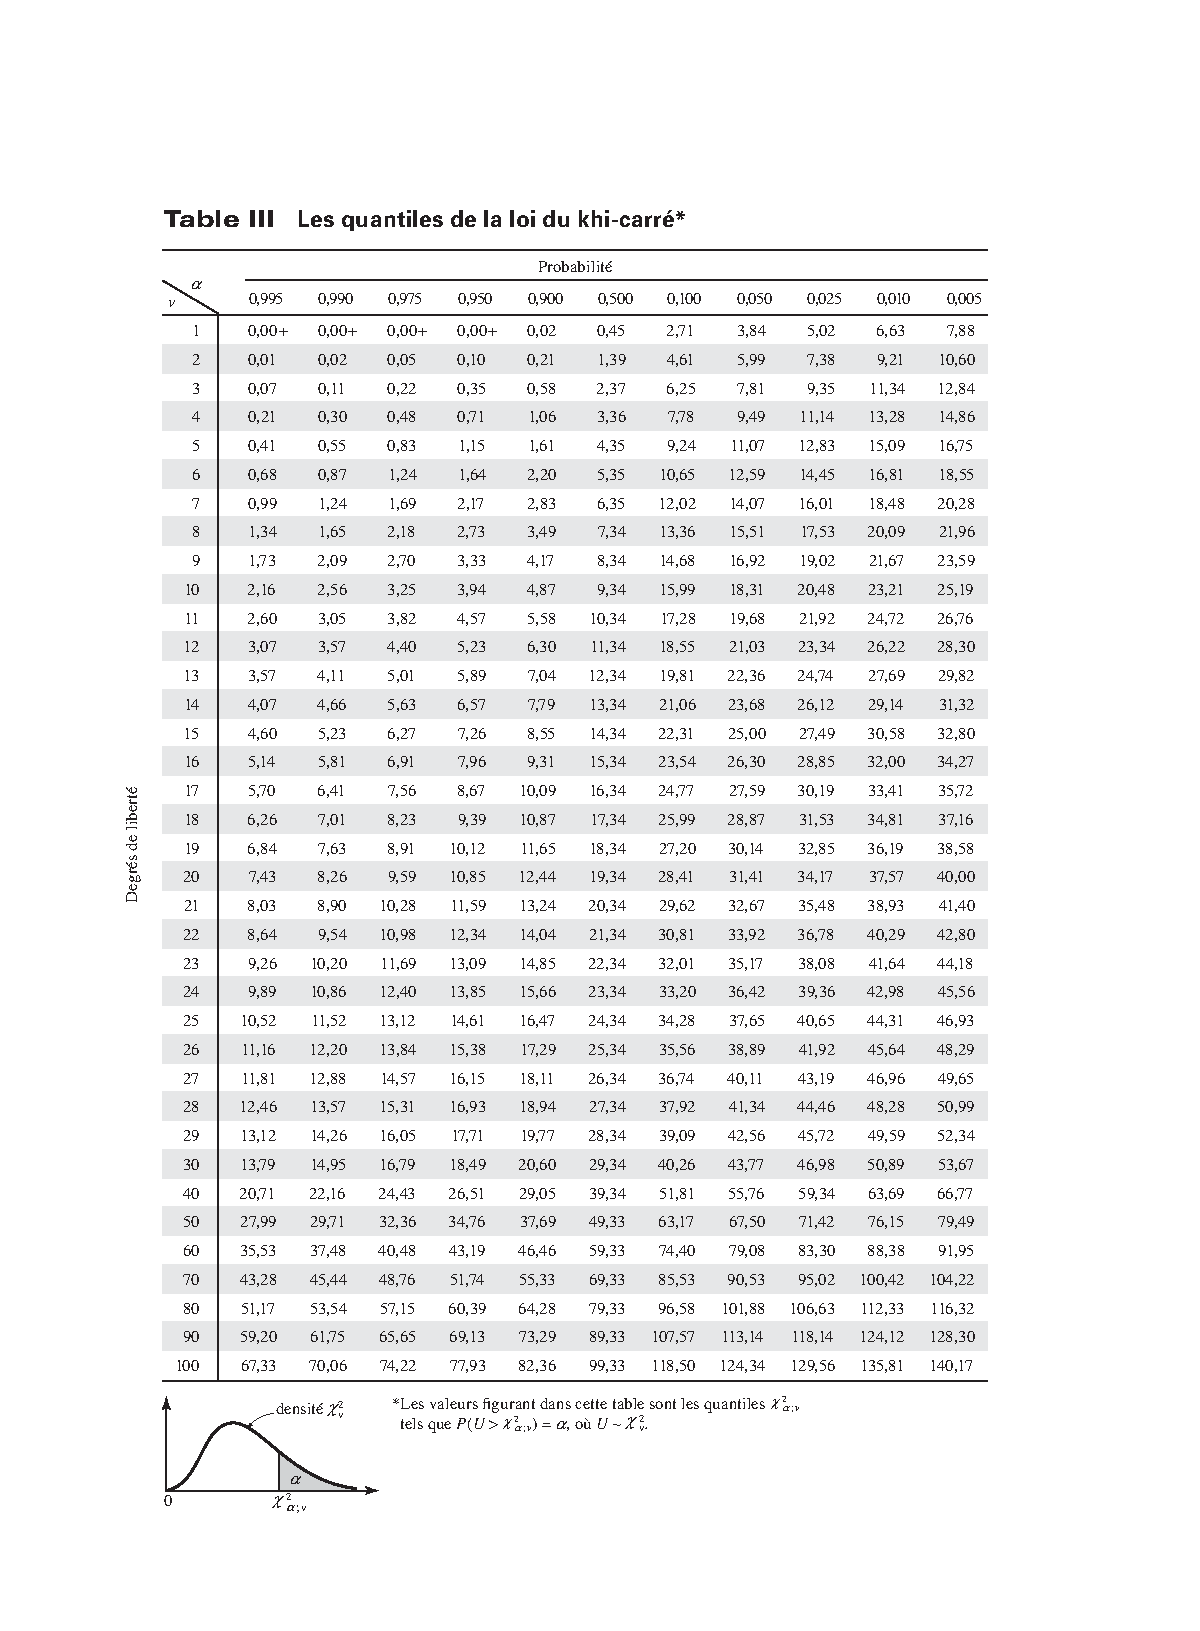
\includegraphics[width=7.6cm]{table_khi2.pdf}} \end{minipage}

\end{frame}
\begin{frame}[t]{Exemple 3}

{\small
\begin{itemize}
\item Supposons que la température d'un four à peinture 30 minutes après l'allumage à $200^{\circ} C$  suit une loi $\mathcal{N}(197, 38)$.
\item Lors de 20 jours différents, on mesure la température après 30 minutes.
\item Quelle est la probabilité que l'écart-type échantillonnal des mesures excède 7,38$^{\circ} C$?
\end{itemize}

\medskip
}
\end{frame}



\section{Loi de Student}

\begin{frame}[t]{Loi de Student (loi $t_v$)}

{\small
\begin{itemize}
\item ressemble  à la $\mathcal{N}(0,1)$, sauf qu'elle a des queues plus lourdes (des
valeurs éloignées de 0 sont plus probables que sous la loi $\mathcal{N}(0,1)$.)
\item un seul paramètre appelé "degrés de liberté" (plus le nombre de degrés de liberté est faible, plus les queues sont lourdes).
    % Si le nombre de degrés de liberté est supérieur à 30, la loi $t$ et la loi $\mathcal{N}(0,1)$ sont presque indistinguables. Ainsi si une v.a. $X$ suit une loi $t$ à $v$ degrés de liberté, on écrit $X\sim t_v$. Sa densité ressemble à ceci :

\end{itemize}
}
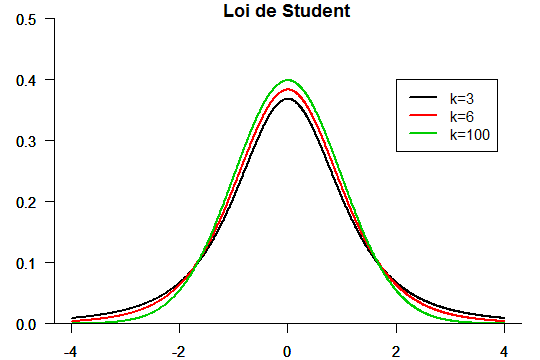
\includegraphics[width=6.5cm]{t.png}

\end{frame}

\only<beamer>{

\begin{frame}{William Sealy Gosset {\it alias} Student}
\begin{tabular}{ccc}
(1876-1937) &Études en chimie & Emploi à Dublin\\

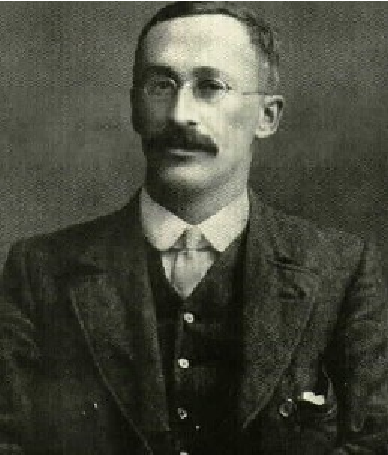
\includegraphics[width=3cm]{Gosset_1.pdf}&
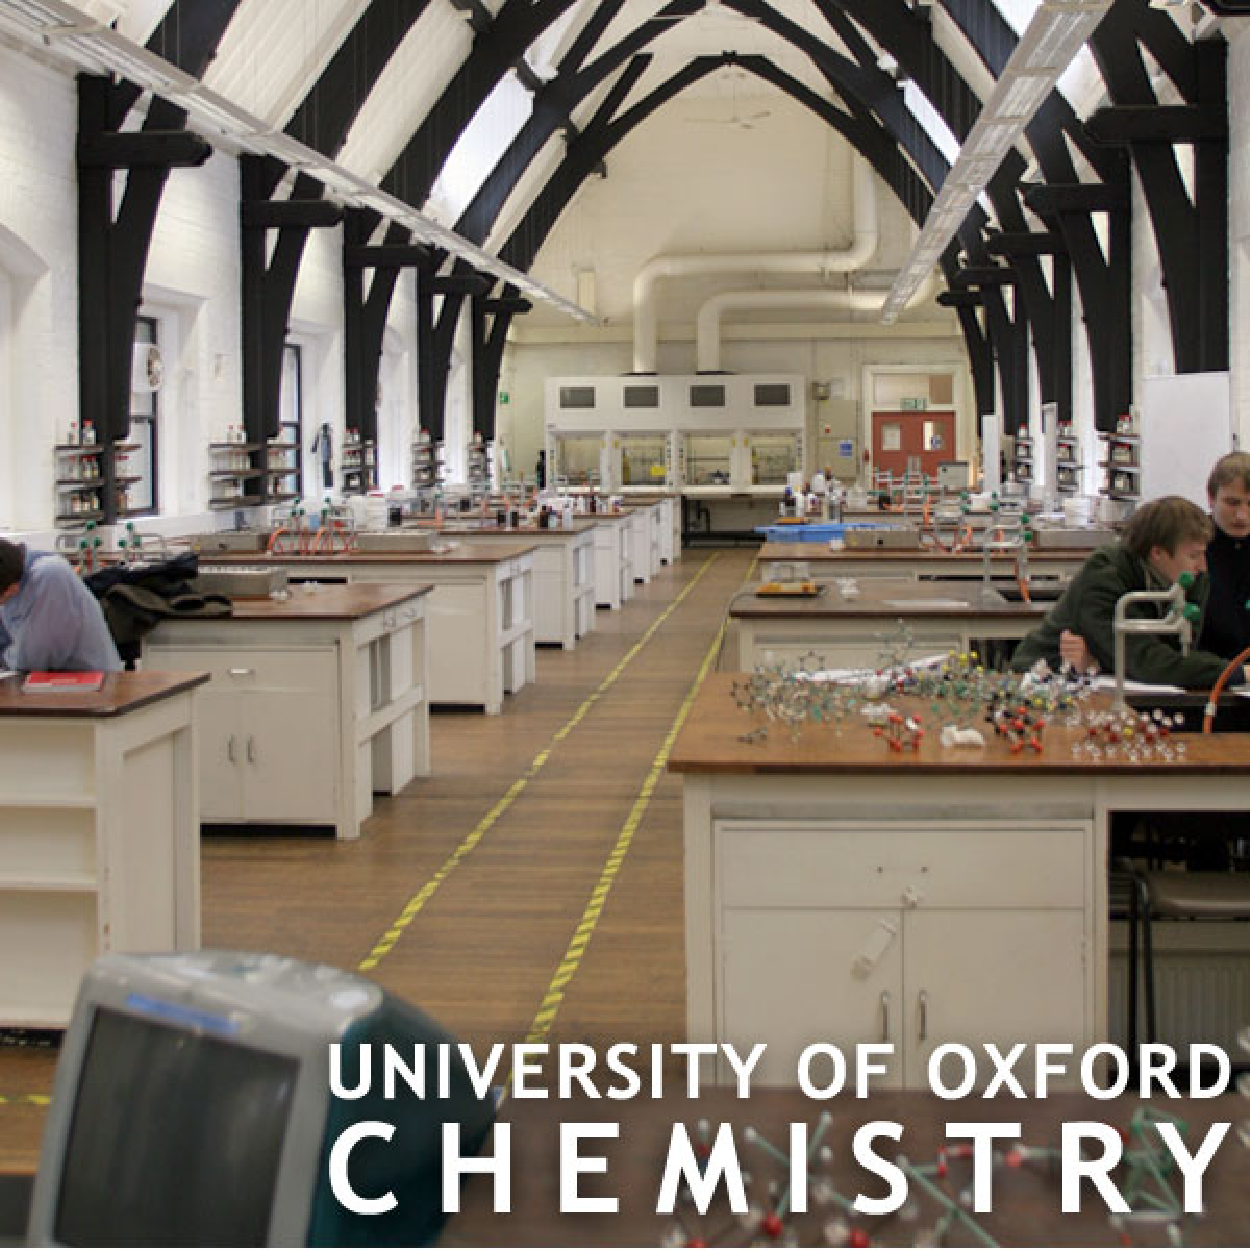
\includegraphics[width=3.5cm]{oxford.pdf}&
\includegraphics[width=3cm]{guinness.pdf}
\end{tabular}
\end{frame}
}
\begin{frame}[t]{Propriétés de la loi $t$}

{\small
\begin{itemize}
\item<1-> Si $T\sim t_v$ {\scriptsize (et $v>1$)}, alors $E(T) = 0$.
\item<1-> Si $T\sim t_v$ {\scriptsize (et $v>2$)}, alors $V(T) = \dfrac{v}{v-2}$.
\item<2-> Si $Z\sim \mathcal{N}(0,1)$, $\quad K\sim\chi^2_v$, $\quad Z$ et $K$ sont indépendantes,
$$\text{alors}\quad \dfrac{Z}{\sqrt{K/v}}\sim t_v$$
\item<3-> Si $X_1,\ldots,X_n$ sont i.i.d. $\mathcal{N}(\mu,\sigma^2)$, alors
$$\frac{\overline{X}-\mu}{S/\sqrt{n}}\sim t_{n-1}.$$
\end{itemize}
}
\end{frame}
\begin{frame}[t]{Table de la loi de Student}

\begin{minipage}[b]{2.5cm}{
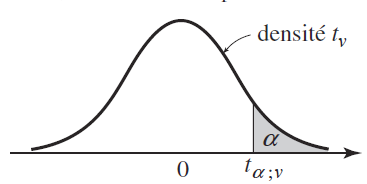
\includegraphics[width=2.5cm]{t-fig.png}

\vspace{9cm}}
\end{minipage}
\begin{minipage}[b]{7.6cm}{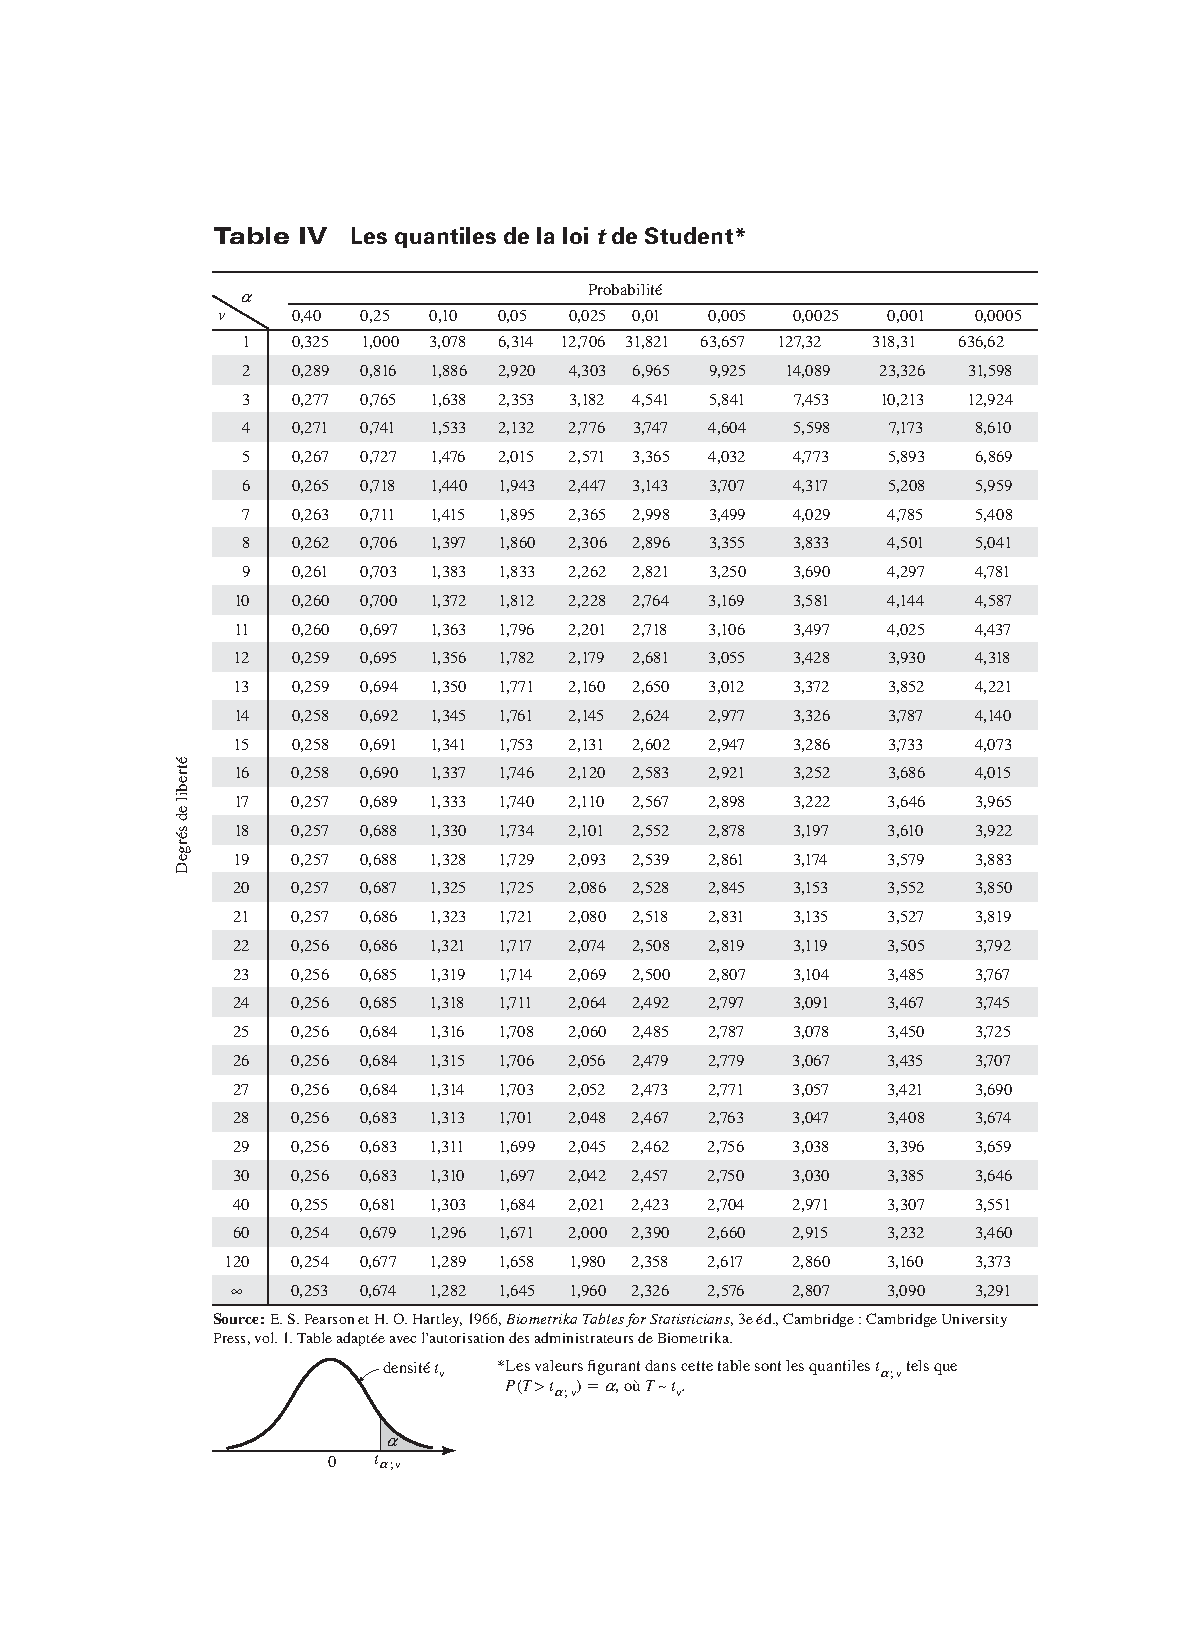
\includegraphics[width=7.6cm]{table_t.pdf}} \end{minipage}

\end{frame}
\begin{frame}[t]{Exemple 4}

{\small
On effectue 9 forages sur un terrain afin de déterminer la
profondeur à laquelle un certain minerai peut être extrait.

\begin{itemize}
\item $X_i=$ profondeur du minerai  lors du forage $i$.
\item On  suppose que les $X_i$ sont i.i.d. $\mathcal{N}(\mu,\sigma^2)$.
    \end{itemize}

Quelle est la probabilité que la moyenne échantillonale soit supérieure à la vraie moyenne $\mu$ par plus d'un écart-type échantillonnal ?

}
\end{frame}



\begin{frame}{Bibliographie}
 	Ce document est rédigé avec Beamer ainsi qu'une classe .cls fourni par Jérôme Soucy. Les diapositives sont adaptées des diapositives créées par Thierry Duchesne et Emmanuelle Reny-Nolin pour le cours STT-1900. Les graphiques proviennent de ces mêmes diapositives.
 	\printbibliography
 	\vfill
 	\footnotesize Pour signaler une erreur dans ce document, veuillez écrire à l'adresse :~\href{mailto:julien.miron@mat.ulaval.ca}{julien.miron@mat.ulaval.ca}.
 \end{frame}

\end{document}

